\documentclass[answers]{exam}
\usepackage{../preamble}
\usepackage{tikz}

\title{Graph Theory -- Sheet 1}
\author{YOUR NAME HERE :)}
\date{Trinity Term 2025}


\begin{document}
\maketitle
\begin{questions}

\question%1
Let $G$ be a connected graph with at least two vertices. Show that there is a vertex $v$ such that $G-v$ is connected. [\emph{You might wish to consider a spanning tree for $G$.}]



\question%2
Let $x$ and $y$ be any two vertices of a tree $T$. Show that there is a unique $x$-$y$ path in $T$.



\question%3
Show that a graph is a tree if and only if it is maximally acyclic.



\question%4
Let $G$ be a graph with $|G|=n$. Show that $G$ is a tree if and only if $G$ is acyclic and $e(G)=n-1$.



\question%5
Let $G$ be a connected graph. Show that any two paths of maximum length intersect.



\question%6
Let $d_{1}, \ldots, d_{n}$ be positive integers. Show that there is a tree on $n$ vertices with vertex degrees $d_{1}, \ldots, d_{n}$ if and only if $\sum_{i=1}^{n} d_{i}=2 n-2$.



\question%7
Consider the weighted graph $G$ depicted below.
\begin{center}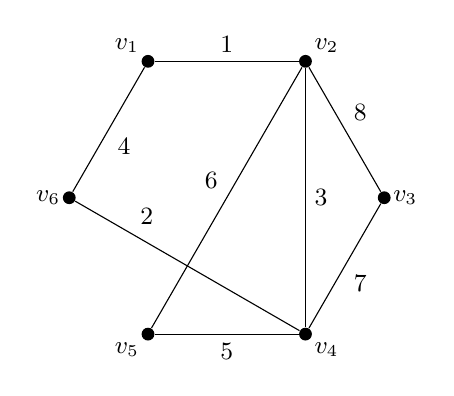
\begin{tikzpicture}
	\begin{scope}[node font=\small]
		\begin{scope}[every node/.style={circle,fill=black,inner sep=0pt,minimum size=.5em}]
			\node (1) at (120:2cm) {};
			\node (2) at (60:2cm) {};
			\node (3) at (0:2cm) {};
			\node (4) at (-60:2cm) {};
			\node (5) at (-120:2cm) {};
			\node (6) at (-180:2cm) {};
		\end{scope}
		
		\node[above left] at (1) {$v_1$};
		\node[above right] at (2) {$v_2$};
		\node[right] at (3) {$v_3$};
		\node[below right] at (4) {$v_4$};
		\node[below left] at (5) {$v_5$};
		\node[left] at (6) {$v_6$};
	
		\path (1) edge node[above] {1} (2);
		\path (1) edge node[below right] {4} (6);
		\path (2) edge node[above right] {8} (3);
		\path (2) edge node[right] {3} (4);
		\path (2) edge node[above left] {6} (5);
		\path (3) edge node[below right] {7} (4);
		\path (4) edge node[below] {5} (5);
		\path (4) edge node[above right,pos=0.75] {2} (6);
	\end{scope}
\end{tikzpicture}\end{center}
\begin{parts}
\part%7a
By applying Kruskal's algorithm, find a minimum cost spanning tree for $G$.

\part%7b
By applying Fleury's algorithm, find an Euler tour for $G$.

\part%7c
Ignoring starting points and orientation, how many Euler tours does $G$ have?
\end{parts}



\question%8
Let $G$ be a connected graph and suppose each edge $e$ has a positive cost $c(e)$. Show that if the costs of the edges are all distinct, then $G$ has a unique minimum cost spanning tree.



\question%9
Let $G$ be a connected graph. Show that $G$ has an Euler trail (i.e. a walk using each edge exactly once) if and only if there are at most two vertices with odd degree.



\question%10
What is the maximum number of edges in a graph on $n$ vertices with no triangle (i.e. no cycle of length 3)?

\end{questions}

\end{document}
